\section{Experimental Evaluation}

    \subsection{Dataset} \label{dataset}
        We have collected 17 videos of both real and synthetically laser machined cracks \comment{(Figure 6.)} The videos are captured by Ahlberg MegaRad L Camera approximately 4-6 inches away from the crack samples moving in a raster scan pattern.  There are 45 unique cracks from all the videos which can differ in length, thickness, and distinguishability and are amoungst various degrees of welding, scratches, and grind marks. Each videos contains approximately 10,000 frames.

    \subsection{Evaluation metric}
        All videos have been manually ground truthed at frame level. Frames containing any part of crack(s) are labeled as true.  As videos have been captured in raster scan, each crack would appear to enter and then exit the video.  The exact time point (frame number) of entry/exit is difficult to determine as only a small part of the crack is visible.  So we ignore  25\% of beginning and ending of the ground truthed entry and exit.
        %For use cross-validation for evaluating method performance by using 16 videos for training for the CNN and plane classification and test on the video left out. We a use frame$-$level classification metric. For each video, frames are marked as crack if any part of a crack appears in the frame. In each crack group described in \ref{planes}, the first 25\% of the frames of the crack group and the last 25\% of the crack group are not used in the frame based evaluation and are labeled as “don’t care”. At these times only a small part of the crack is visible, and the crack usually can not be clearly distinguished.
        For each video, the true positive rate (TPR), the false positive rate (FPR) and the F1-score are computed where TP, FP, TN, FN are deteremined at frame-level.
        
        %  \begin{itemize}
        %    \item  $TPR = TP / (TP + FN)$
        %    \item  $FPR = FP / (FP + TN)$
        %    \item  $F1 = (2 * TP) / (2 * TP + FP + FN)$
        %\end{itemize}
        
        %A crack classified frame is TP if any patch in the frame is detected as crack and the ground truth is labeled crack, or FP otherwise. A non$-$crack classified frame is TN if no patches in the frame are detected as crack and the ground truth is labeled non-crack, or FN otherwise. We use True Positive Rate (TPR), False Positive Rate (FPR), and F1-Score to evaluate performance at the frame level. If TP, FP, TN, and FN represent the total number of frames classified as such, then: 
      
    
        \begin{table}
        
            \begin{center}
            
                \begin{tabular}{ l c|c|c| }\\
                    \hline
                        \multicolumn{1}{|l||}{\textbf{Method}} & \textbf{TPR} & \textbf{FPR} & \textbf{F1}\\
                    \hline
                        \multicolumn{1}{|p{2cm}||}{Without Spatio-Temporal} & 0.79 & 0.02 & 0.79 \\
                    \hline
                        \multicolumn{1}{|p{2cm}||}{With Spatio-Temporal} & 0.86 & 0.04 & 0.81 \\
                    \hline
                \end{tabular}
                
                \caption{Frame-level evaluation }
                \label{ResultsFrame}
            
            \end{center}
            
        \end{table}
        
        
        %% ------------------------------------------------
        %   Our dataset method Comparison Examples:
        %% ------------------------------------------------
        \begin{figure*}
        
            \begin{centering}
                \begin{tabular}{c|c|c}
                    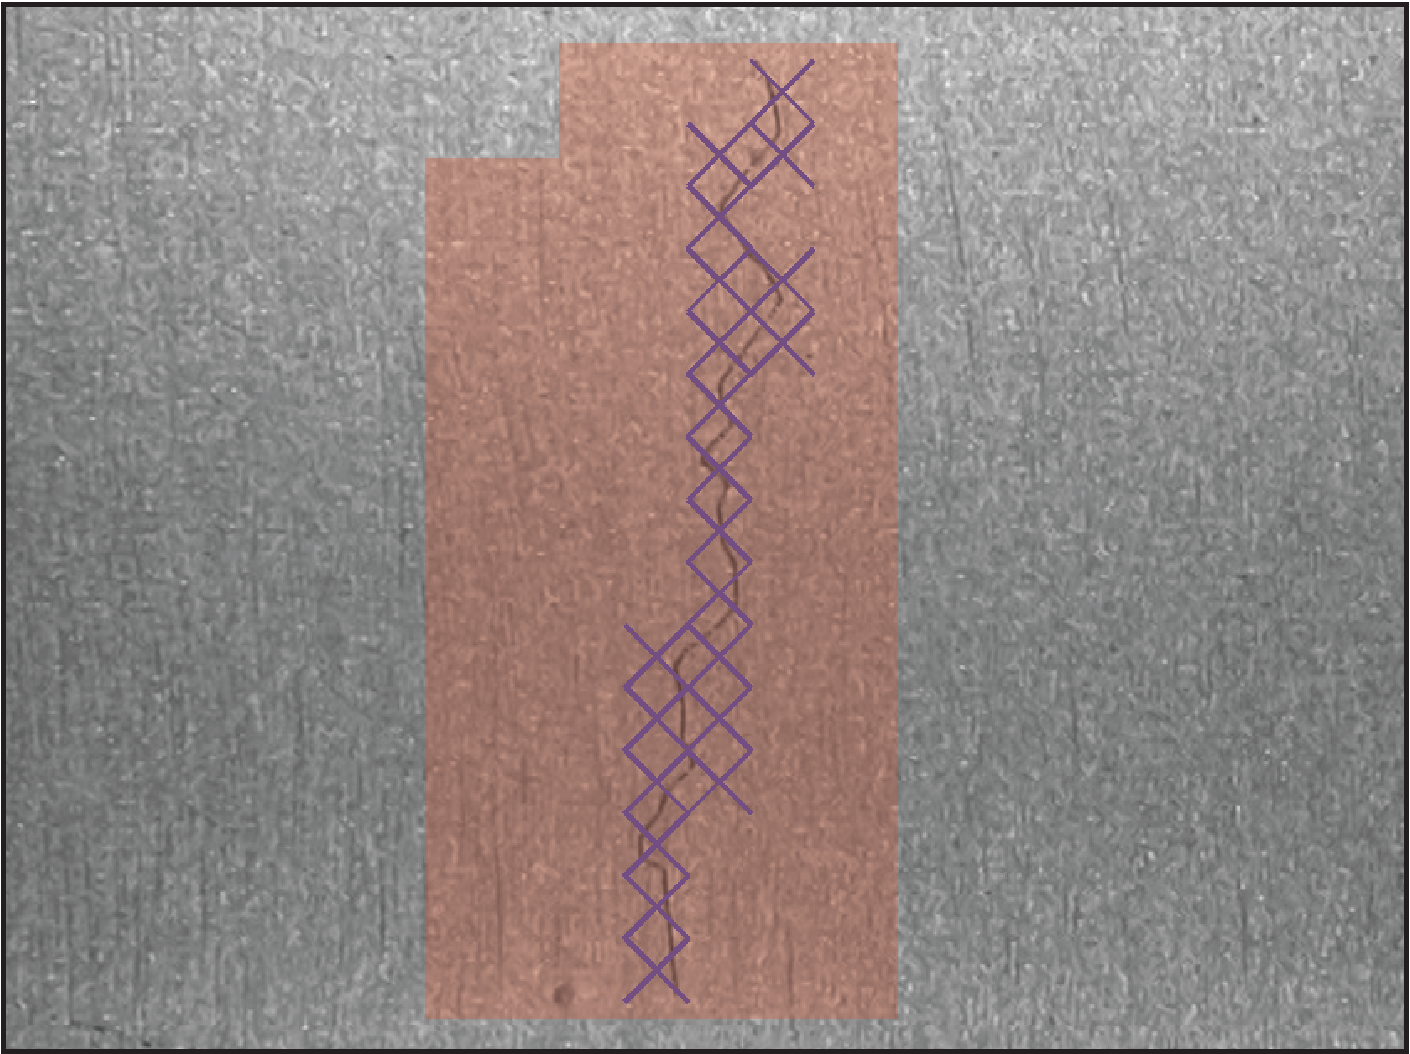
\includegraphics[width=0.3\textwidth]{Images/TP_All_2.pdf} & 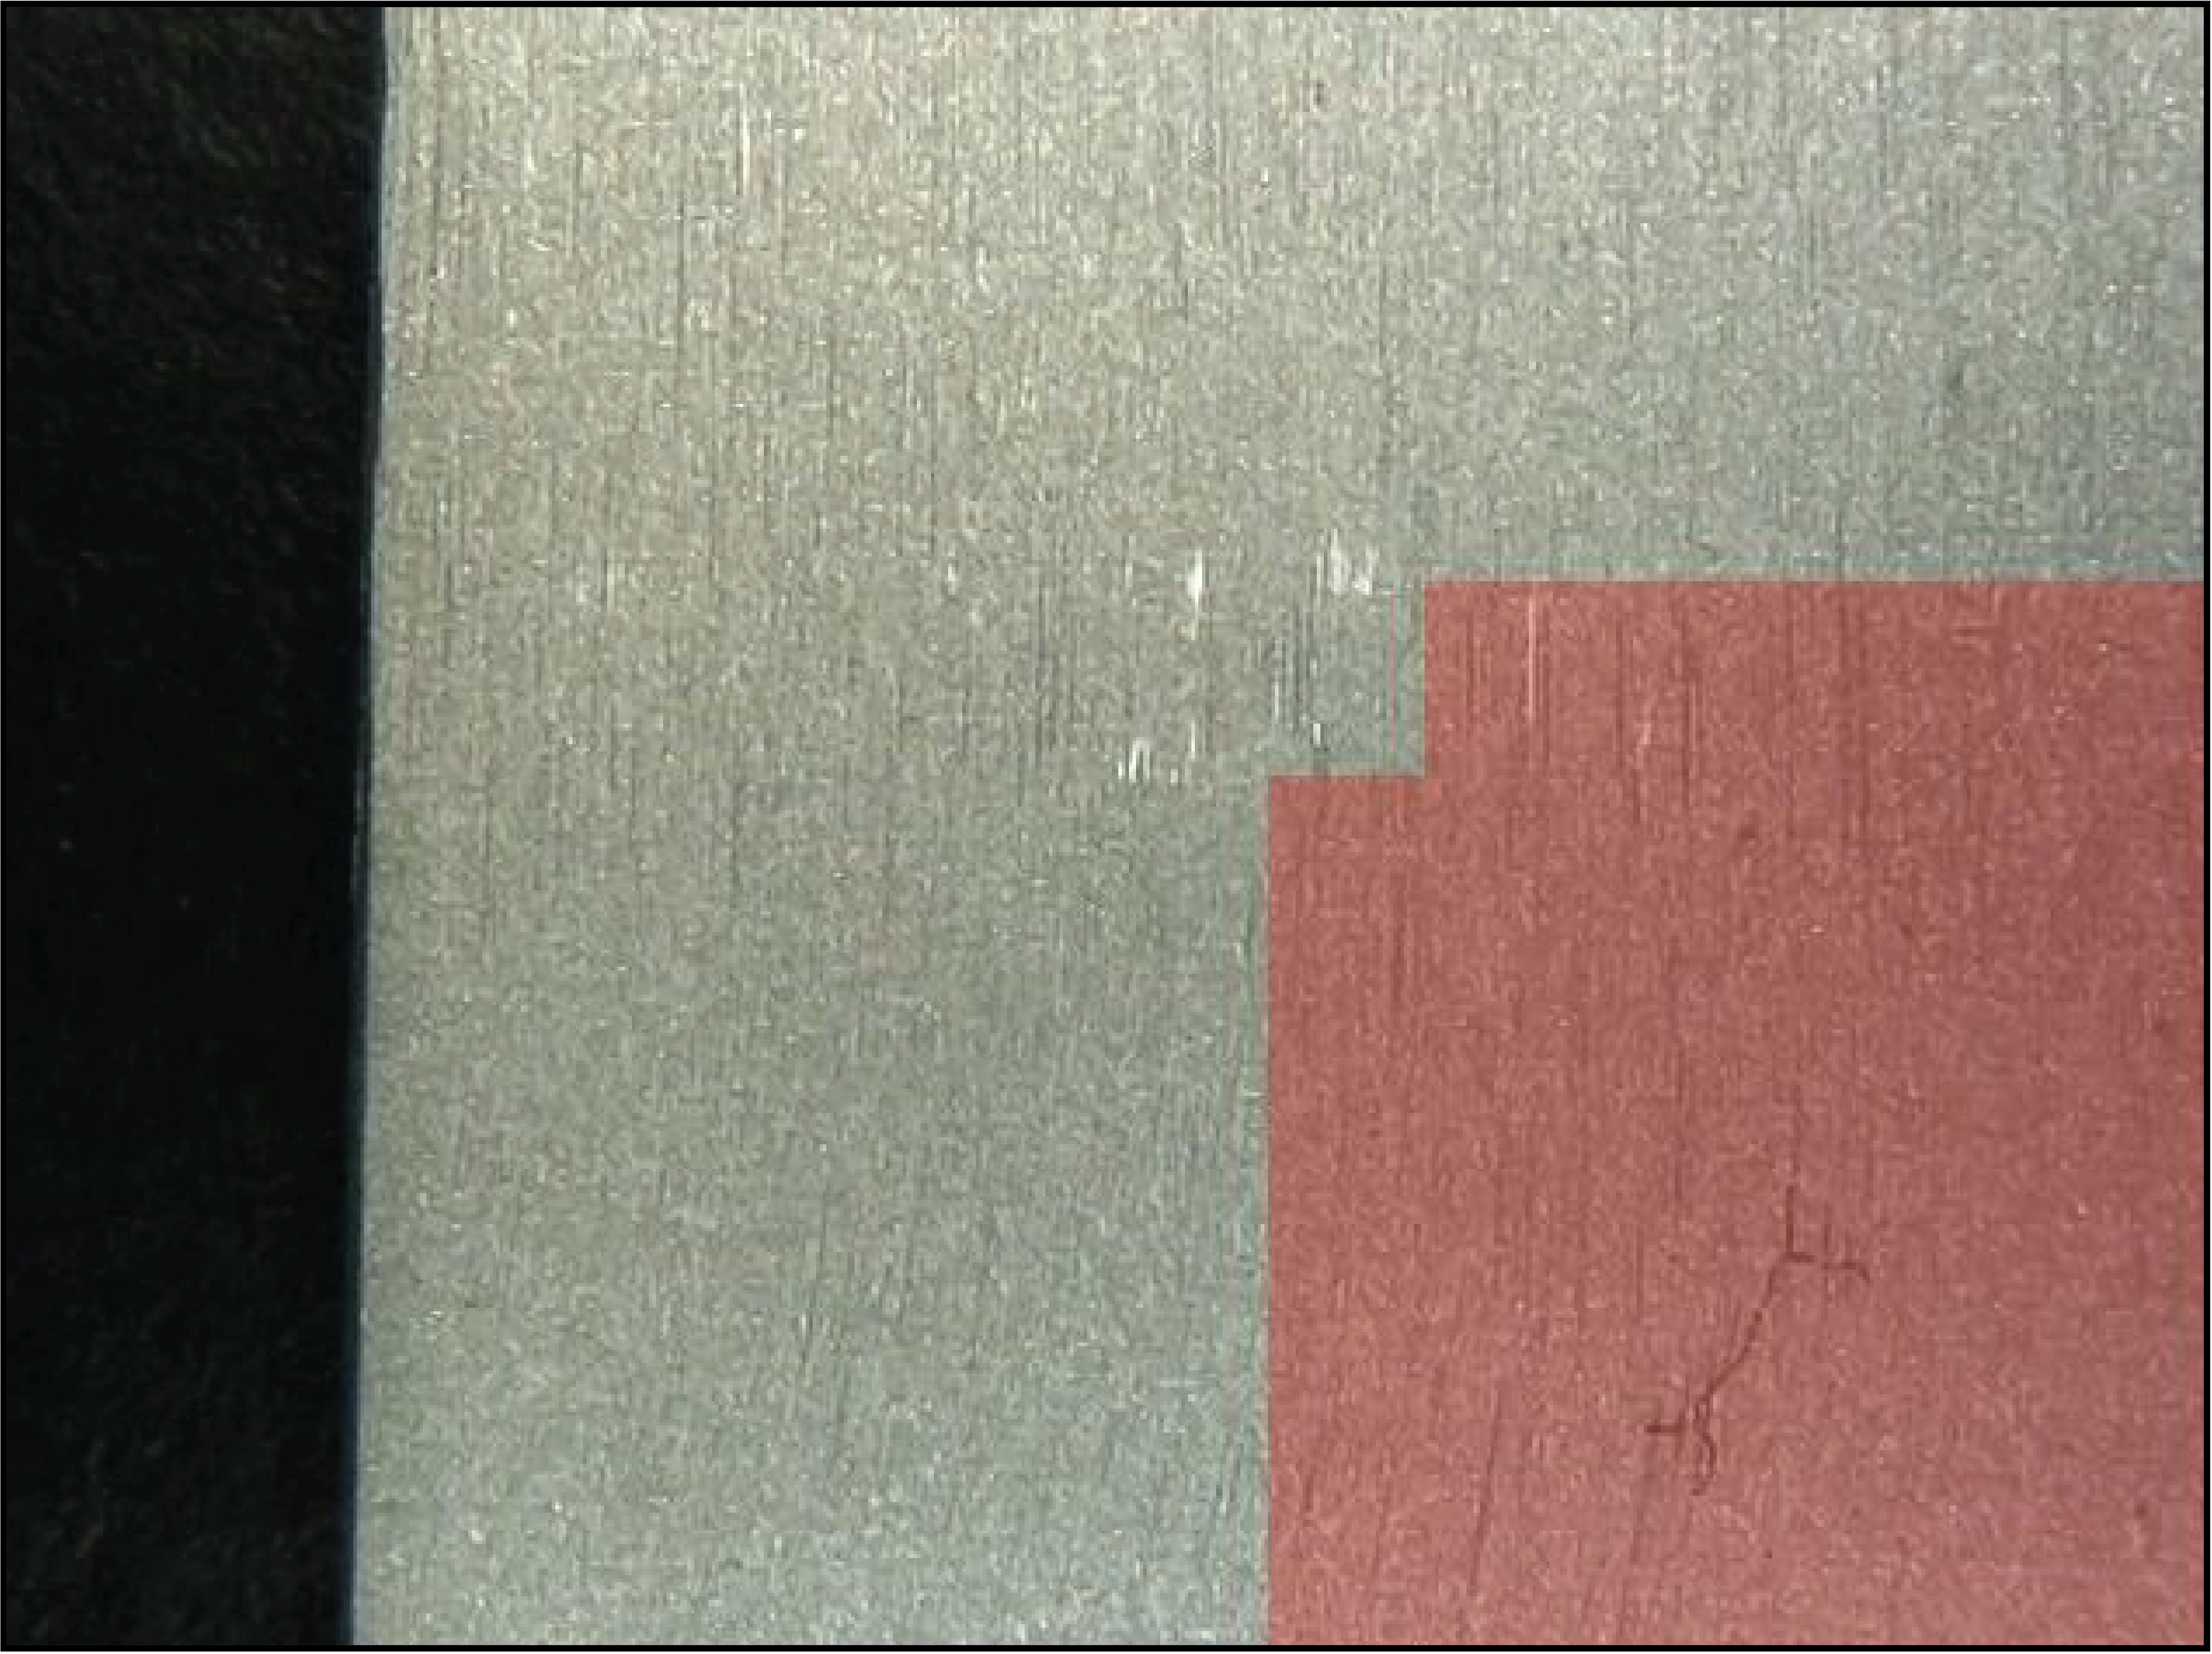
\includegraphics[width=0.3\textwidth]{Images/TP_us_FN_them_2.png} &
                    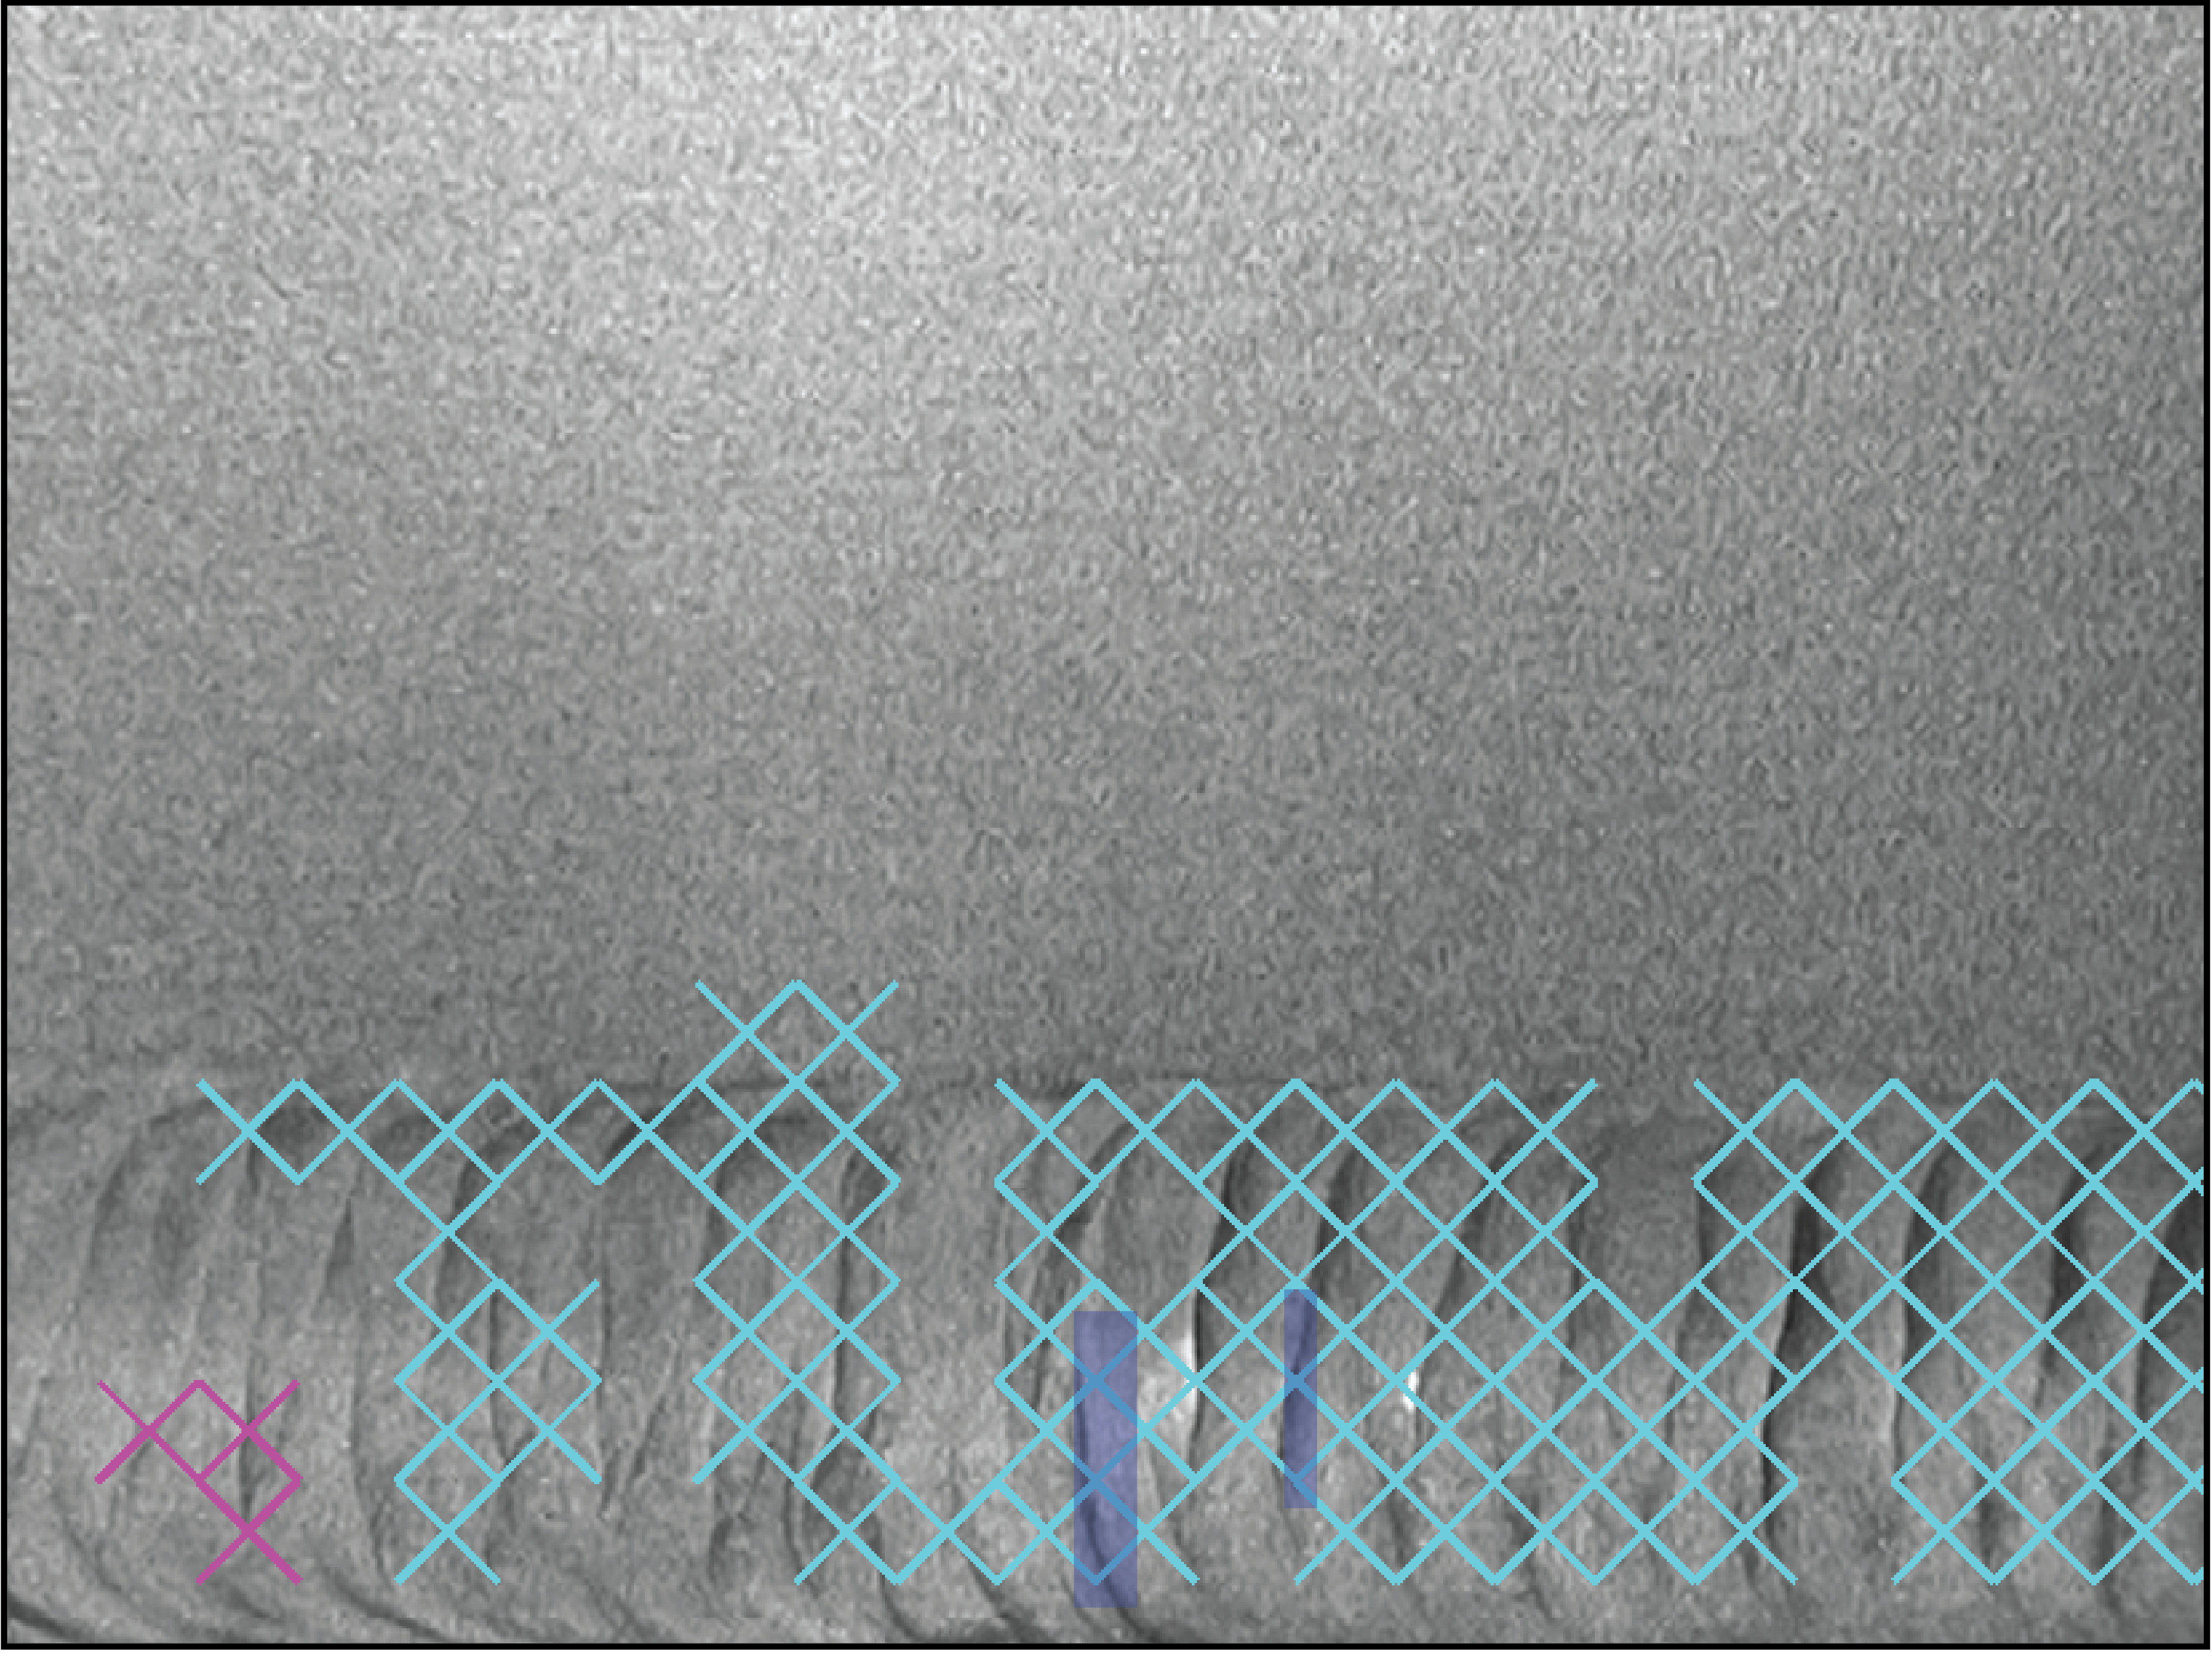
\includegraphics[width=0.3\textwidth]{Images/FP_others_2.png} \\
                    (a) TP by all methods & (b) FN by other methods & (c) FP by other method \\
                \end{tabular}
                
                \caption{Our dataset comparison with others. first is all TP, second is TP us and FN them, third is TP us and FP them. I can make them look better later.}
                \label{plantCompareExamples}
                 
            \end{centering}
            
        \end{figure*}
        %% ------------------------------------------------
        
        
        %% ------------------------------------------------
        %   CrackIT dataset method Comparison Examples:
        %% ------------------------------------------------
        \begin{figure*}
        
            \begin{centering}
                \begin{tabular}{c|c}
                    \includegraphics[width=0.45\textwidth]{Images/CrackIT_TP_All-2.png} & \includegraphics[width=0.45\textwidth]{Images/CrackIT_FP_ByCrackIT-2.PNG} \\
                     \\
                    (a) True crack frame detection by all methods & (b) Incorrect crack frame detection by CrackIT
                \end{tabular}
                
                \caption{TODO: figure explaination...}
                \label{crackitExamples}
                 
            \end{centering}
            
        \end{figure*}
        %% ------------------------------------------------
        
        
        %% ------------------------------------------------
        %                 Results Table
        %% ------------------------------------------------
        \begin{table}
        
            \begin{center}
            
                \begin{tabular}{ l c|c|c| }\\
                    \hline
                        \multicolumn{1}{|l||}{\textbf{Method}} & \textbf{TPR} & \textbf{FPR} & \textbf{F1}\\
                    \hline
                        \multicolumn{1}{|p{2cm}||}{CNN} & 0.75 & 0.03 & 0.79 \\
                    \hline
                        \multicolumn{1}{|p{2cm}||}{CrackIT} & 0.79 & 0.60 & 0.33 \\
                    \hline
                        \multicolumn{1}{|p{2cm}||}{Morph} & 0.47 & 0.19 & 0.39 \\
                    \hline
                \end{tabular}
                
                \caption{Results comparison on power plant crack dataset. 346 images (0.25\% of entire frames of dataset) are used to compare performance between algorithms. A frame based evaluation is used. If any blocks in the image are classified as crack, the image is classified as having a crack. CrackIT uses training learned from road crack dataset. The input image resolution size was tuned for the CrackIT algorithm to account for the smaller size image and smaller thickness of nuclear cracks.}  
                \label{ResultsComparisonNuclearDataSet}
            
            \end{center}
            
        \end{table}
        
        \begin{table}
        
            \begin{center}
            
                \begin{tabular}{ l c|c|c| }\\
                    \hline
                        \multicolumn{1}{|l||}{\textbf{Method}} & \textbf{TPR} & \textbf{FPR} & \textbf{F1}\\
                    \hline
                        \multicolumn{1}{|p{2cm}||}{CNN} & 1.00 & 0.00 & 1.0 \\
                    \hline
                        \multicolumn{1}{|p{2cm}||}{CrackIT} & 1.00 & 0.25 & 0.98 \\
                    \hline
                        \multicolumn{1}{|p{2cm}||}{Morph} & 1.00 & 0.00 & 1.00 \\
                    \hline
                \end{tabular}
                
                \caption{Results comparison on CrackIT road crack dataset. 48 images (40 crack images 8 non-crack) are used to compare performance between algorithms. A frame based evaluation is used. If any blocks in the image are classified as crack, the image is classified as having a crack. CNN is trained from nuclear power plant dataset. CNN block size was tuned and found to do best with 171x171 block size. A different block size is necessary for CNN to account for the higher resolution of images and the  greater thickness of road cracks.   }
                \label{ResultsComparisonRoad}
            
            \end{center}
            
        \end{table}
        
        %% ------------------------------------------------
        
        
        % \paragraph{Crack-level}
        %     We also evaluate at the crack camera pass level. We use an overlap strategy based on \\cite{HooverGoldgofpaper}. GT Crack groups are created from frames that are consecutively labeled as cracks. GT non-crack groups are created from consecutive frames labeled as non-cracks.  For each crack detected plane interval and GT Crack Group combination, the number of frames of overlap is computed and then the $overlap-percentage = \min( percent-frame-Overlap-with-GT, percent-frame-Overlap-with-detection)$ is computed.   Each GT Crack group is matched to the crack detection group with the highest overlap-percentage if the $overlap-percentage >= 0.1$. This is then counted as a TP.  Each GT Crack Group can only be matched to one crack detection group. 
        %     FNs are the number GT Crack groups that do not get matched to a crack group detection. 
        %     FPs are the number of crack group detections that do not get matched to a GT Crack group.
        %     TNs are the number GT non-crack groups that get matched to non-crack groups from detection using similar overlap criteria as TPs. 

    \subsection{Accuracy}

        \paragraph{Spatial$-$temporal grouping performance}
            We first evaluate the effectiveness of spacial$-$temporal grouping. Table \ref{ResultsFrame} compares the proposed method with and without spatial$-$temporal grouping. 
            Classification of crack frames using only individual image patches (i.e. without spatial$-$temporal grouping) achieved a TPR just under 80\% and a low FPR of 2\%. The addition of spacial$-$temporal grouping improved the TPR of crack frame classification by 8\% with a negligible increase in FP detections for an overall improvement in F1 measure.   
            \comment{The improvoment is mostly on TPRs, the most of benefits is due to better identification of begining and ending of the crack durations. I'm STILL THINKING} 
            

        \paragraph{Comparison with related works}
            Previous works CrackIT \comment{[X]} and Morph \cite{jahanshahi2013} were compared against on two datasets: 1) the nuclear power plant crack data set described in \ref{dataset}, and 2) the pavement crack data set presented in the CrackIT work. The CrackIT method is publicly availble and trained with data from their pavement crack data set. For the power plant data set the input image resolution size was better tunned for the CrackIT algorithm to account for the smaller image size and thickness of nuclear plant cracks. The Morph method was implemented to follow \cite{jahanshahi2013} as closely as possible. For training the artificial neural network of the Morph method, we used both actual and synthetically generated positive and negative examples of cracks nuclear power plants as the process describes in their work.  Please note that we only compare the results of the proposed method without spacial$-$temporal grouping for a better comparison with the related works and that only 0.25\% of the frames were used for this method comparison. 
            
            Table \ref{ResultsComparisonNuclearDataSet} shows the results of each method for crack frame classification on the nuclear power plant data set. The CrackIT method showed a slight improvement over the proposed method only in terms of TPR, but also had a large performance drop in FPR resulting in the lowest F1 score of the methods compared.  The proposed method displayed the best F1 score by a considerable margin over the other methods.  \comment{We need to add why and link to what's unique about our method.  Since this does not involve grouping, this has to be all about convNN performance.  Our method uses much larger area for computing features and uses (convNN) 224x224 pixel (I think that other two methods uses much smaller window, Steve can check this).  Also, morph method classifies each connected component based on geometric features.  In our dataset, the difference between crack and non-crack in geometry is very subtle}
            
            For pavement crack data set \comment{[X}}, Table \ref{ResultsComparisonRoad} shows the performance of each of the methods for frame crack classification. For the proposed method on the pavement crack data set, image patches of size 171$x$171, which were still resized into 224$x$224 to input to the CNN, were used to account for the smaller image sizes of the data set.  \comment{talk about training of the methods}
            By the perfect performance scores of both the proposed and Morph method, we can tell that the data set is considerably less difficult. This can also we qualitatively confirmed by visual inspection of the data set images, for example \ref{crackitExamples}. 
            
            
        
        
        
        
